\begin{frame}
	\centering
	\fontsize{22pt}{24pt}\selectfont
	Inovação Disruptiva e Ambidesteridade
\end{frame}

\begin{frame}{Referências}
    \begin{vfilleditems}
    \footnotesize
    \item \fullcite{christensen2015disruptive} (\textcolor{red}{Conceitual, revista mais voltada para prática HBR})
    \item \fullcite{march1991exploration} (\textcolor{red}{Conceitual, seminal})
    \item \fullcite{tushman1996ambidextrous} (\textcolor{red}{Conceitual, seminal})
    \item \fullcite{gibson2004antecedents}
	    (\textcolor{red}{Empírico, uma das evidências mais relevantes da teoria, amostragem boa})
    \item \fullcite{raisch2008organizational}
	    (\textcolor{red}{Conceitual, uma baita revisão da literatura com uma proposta de framework})
    \end{vfilleditems}
\end{frame}

\begin{frame}{Inovação Disruptiva}
    \begin{vfilleditems}
    \item Todo mundo usa inovação disruptiva, sem ler um único livro ou artigo científico sobre o tema
    \item Usam erroneamente para qualquer situação em que um setor seja abalado e os líderes anteriores não conseguem manter seu sucesso
    \end{vfilleditems}
\end{frame}

\begin{frame}{Inovação Disruptiva}
    \begin{vfilleditems}
    \item \textbf{Inovações disruptivas} são originárias em baixo custo ou em novos mercados
    \item \textbf{As inovações disruptivas} não alcançam os clientes comuns até que a qualidade atenda aos seus padrões
    \end{vfilleditems}
\end{frame}

\begin{frame}{Inovação Disruptiva}
	\centering
	\begin{figure}
	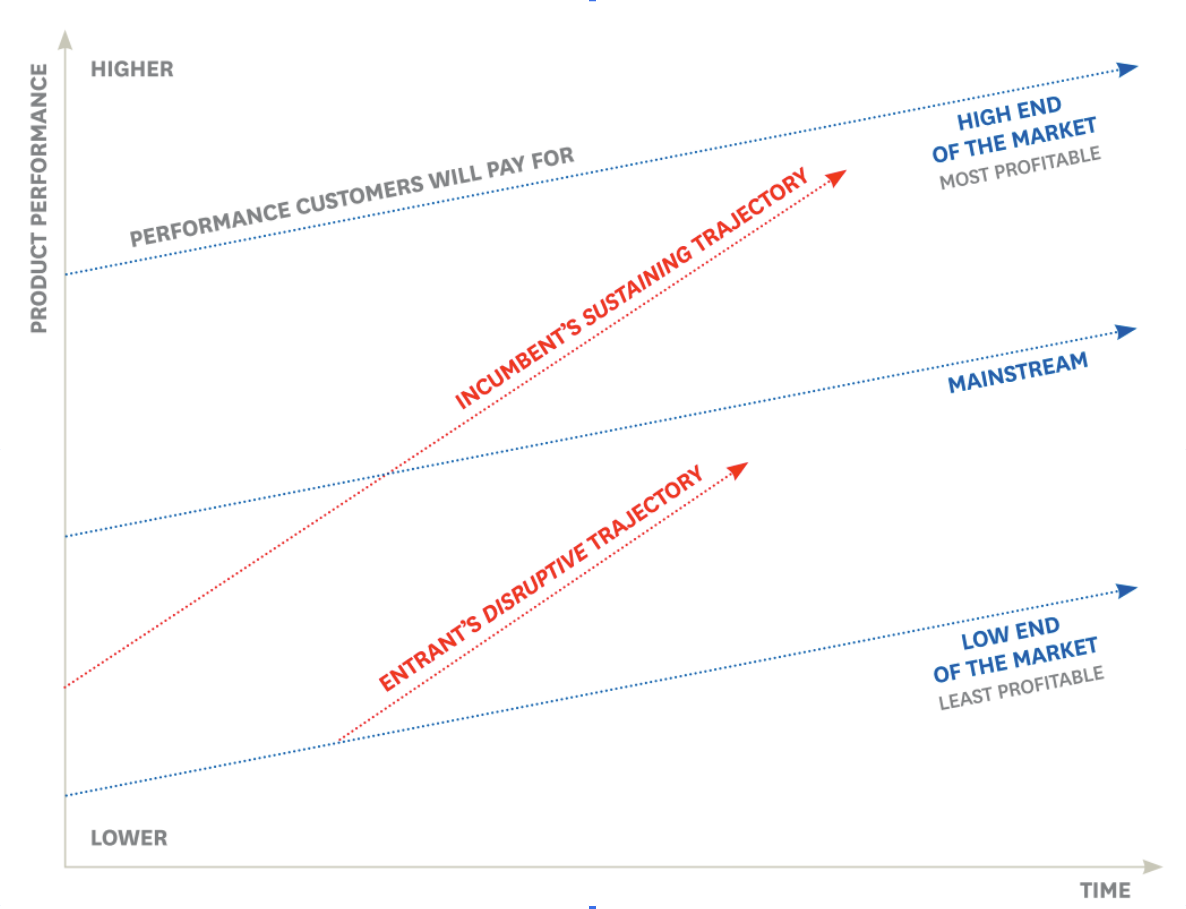
\includegraphics[width=0.55\textwidth]{inov_disruptiva.png}
	\caption{Inovação Disruptiva. Fonte: \textcite{christensen2015disruptive}.}
	\label{fig:inov_disruptiva}
	\end{figure}
\end{frame}

\begin{frame}{Uber é uma Inovação Disruptiva?}
	\centering
	
\includegraphics[width=0.30\textwidth]{meme_sim_nao.jpg}
\end{frame}

\begin{frame}{4 pontos-chave da Teoria de Inovação Disruptiva}
    \begin{vfilleditems}
    \item[1] \textbf{Disrupção é um processo}: não deve ser usado para se referir a um
	    produto ou serviço em um ponto fixo, mas para a evolução desse produto
	    ou serviço ao longo do tempo.
    \end{vfilleditems}
\end{frame}

\begin{frame}{4 pontos-chave da Teoria de Inovação Disruptiva}
    \begin{vfilleditems}
    \item[2] \textbf{Disruptores geralmente criam modelos de negócio bem diferentes daqueles já existentes.}
    \end{vfilleditems}
\end{frame}

\begin{frame}{4 pontos-chave da Teoria de Inovação Disruptiva}
    \begin{vfilleditems}
    \item[3] \textbf{Algumas inovações disruptivas obtém sucesso outras não}: 
	    miopia de se focar em resultados alcançados
    \end{vfilleditems}
\end{frame}

\begin{frame}{4 pontos-chave da Teoria de Inovação Disruptiva}
    \begin{vfilleditems}
    \item[4] \textbf{O mantra “Be disruptive or be disrupted” pode ser enganoso}:
	    As empresas existentes precisam responder à disrupção, se estiver ocorrendo,
	    mas não devem exagerar ao desmantelar um negócio ainda lucrativo. Em vez disso,
	    eles devem continuar a fortalecer o relacionamento com os principais clientes,
	    investindo na sustentação de inovações.
    \end{vfilleditems}
\end{frame}

\begin{frame}{Ambidesteridade - \textit{Exploitation}/\textit{Exploration}}
	\begin{table}[]
	{\small
	\centering
	\begin{tabularx}{\textwidth}{|l|X|X|}
	\hline
	                                & \textbf{Exploitation}                        & \textbf{Exploration}                             \\ \hline
	\textbf{Intenção Estratégica}   & Custo, lucro                                 & Inovação, crescimento                            \\ \hline
	\textbf{Tarefas Críticas}       & Operações, eficiência, inovação incremental  & Adaptação, novos produtos, inovação radical      \\ \hline
	\textbf{Competências}           & Operacional                                  & Empreendedora                                    \\ \hline
	\textbf{Estruturas}             & Formal, mecanicista                          & Adaptativa, orgânica                             \\ \hline
	\textbf{Controles, recompensas} & Margens, produtividade                       & Marcos, crescimento                              \\ \hline
	\textbf{Cultura}                & Eficiência, baixo risco, qualidade, clientes & Risco, velocidade, flexibilidade, experimentação \\ \hline
	\textbf{Papel da liderança}     & Autoritativa, de cima para baixo             & Visionária, envolvida                            \\ \hline
	\end{tabularx}}%
	\end{table}	
\end{frame}

\begin{frame}{Ambidesteridade Estrutural e Contextual}
    \begin{vfilleditems}
    \item \textbf{Estrutural}: as organizações gerenciam trade-offs
	    entre demandas conflitantes, criando "estruturas duplas",
	    para que determinadas unidades de negócios - ou
	    grupos dentro de unidades de negócios - se concentrem no
	    alinhamento, enquanto outras se concentram na adaptação
    \end{vfilleditems}
\end{frame}

\begin{frame}{Ambidesteridade Estrutural e Contextual}
    \begin{vfilleditems}
    \item \textbf{Contextual}: a capacidade comportamental de demonstrar
	    simultaneamente alinhamento e adaptabilidade em
	    toda uma unidade de negócios
    \end{vfilleditems}
\end{frame}

\begin{frame}{Ambidesteridade e Desempenho}
	\begin{figure}
		\centering
		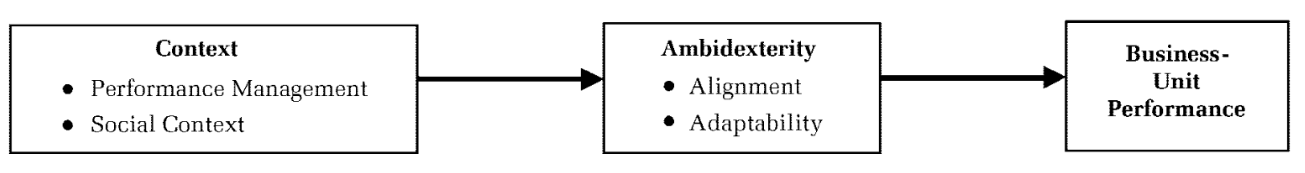
\includegraphics[width=1.0\textwidth]{ambidex_performance.png}
		\caption{Contexto, Ambidesteridade e Desempenho. Fonte: \textcite{gibson2004antecedents}.}
		\label{fig:ambidex_performance}
	\end{figure}
\end{frame}

\begin{frame}{\textcite{gibson2004antecedents}}
	\begin{vfilleditems}
	\item \textbf{Amostra}: 4,195 indivíduos de 41 unidades de negócio em 10 empresas multinacionais
	\item \textbf{Escala Likert} de 7 pontos: Discordo-Concordo
	\item \textbf{Variável Dependente}: Desempenho
	\item \textbf{Variável Mediadora}: Ambidesteridade
		\begin{vfilleditems}
		\item Alinhamento
		\item Adaptabilidade
		\end{vfilleditems}
	\item \textbf{Variável Independente}: Contexto Organizacional
		\begin{vfilleditems}
		\item Gestão de Desempenho
		\item Contexto Social
		\end{vfilleditems}
	\item \textbf{Variáveis de Controle}: \textit{dummy} para cada multinacional	
	\end{vfilleditems}
\end{frame}

\begin{frame}{\textcite{gibson2004antecedents}}
	\begin{figure}
		\centering
		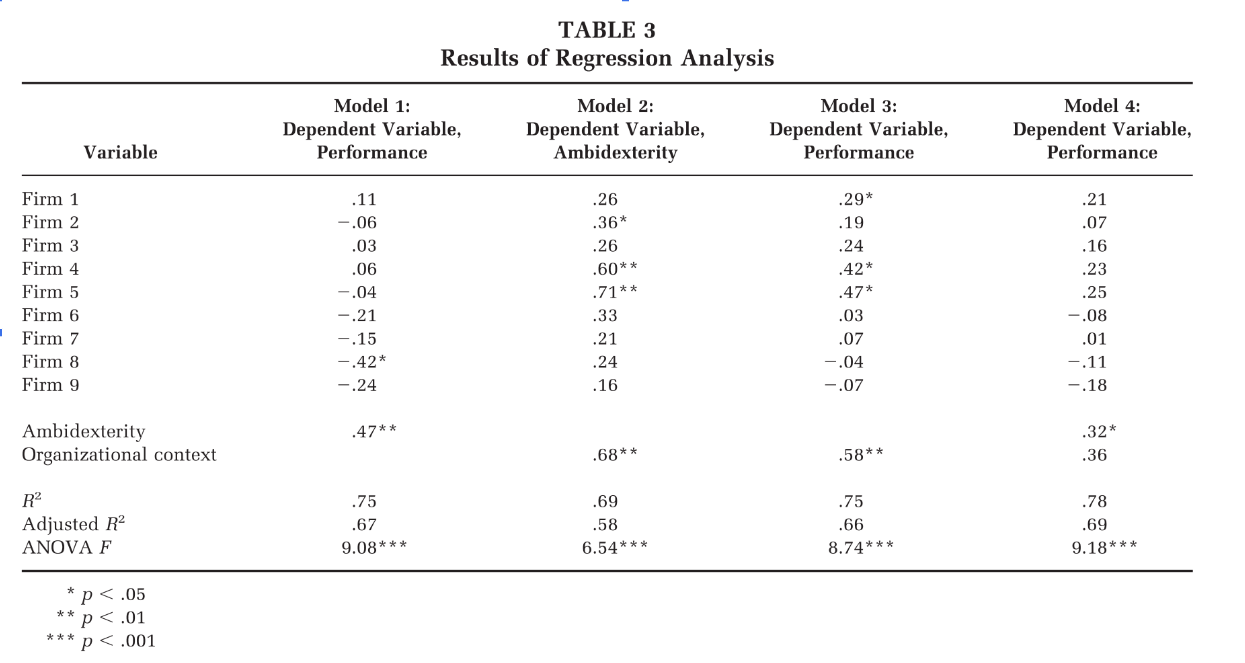
\includegraphics[width=0.8\textwidth]{ambidex_results.png}
		\caption{Resultados das Regressões. Fonte: \textcite{gibson2004antecedents}.}
		\label{fig:ambidex_results}
	\end{figure}
\end{frame}

\begin{frame}{\textcite{raisch2008organizational}}
	\begin{figure}
		\centering
		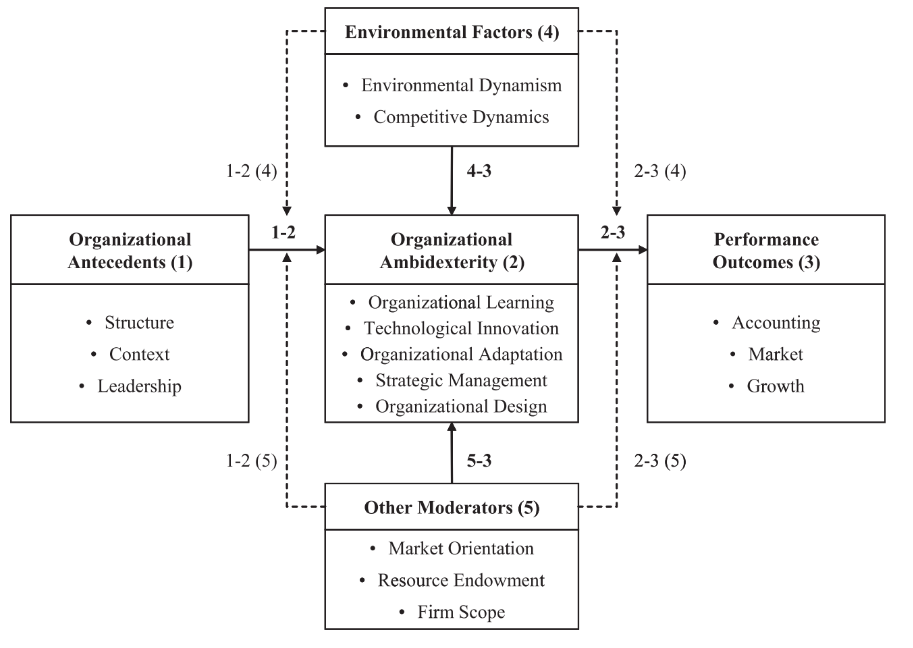
\includegraphics[width=0.6\textwidth]{ambidex_model.png}
		\caption{Modelo de Ambidesteridade Organizacional. Fonte: \textcite{raisch2008organizational}.}
		\label{fig:ambidex_model}
	\end{figure}
\end{frame}

